\section{Climate Change Sparks Civil Unrest}
The environmental changes from climate change can have important effects on our well-being and security. Reduction of arable land, widespread shortage of water, diminishing food and fish stocks, increased flooding and prolonged droughts are already happening in many parts of the world. A drop in agricultural productivity will lead to, or worsen, food-insecurity in least developed countries and an unsustainable increase in food prices across the board. Water shortage in particular has the potential to cause civil unrest and to lead to significant economic losses. Those parts of the populations that already suffer from poor health conditions, unemployment or social exclusion are rendered more vulnerable to the effects of climate change, which could amplify or trigger migration within and between countries. Climate change may significantly increase instability in weak or failing states by over-stretching the already limited capacity of governments to respond effectively to the challenges they face. One of the most significant potential conflicts over resources arises from intensified competition over access to, and control over, energy resources. That in itself is, and will continue to be, a cause of instability.

While it is unlikely that the physical impacts of climate change will have a direct effect on conflict, there are a number of plausible causal mechanisms that run through intermediate variables, such as population exposure and human health, economic growth, institutional capacity and governance, and other known conflict predictors. Additionally, there is growing consensus that the anticipated physical effects of climatic changes will have serious implications for human wellbeing and security, but quantitative efforts to assess how the impacts will influence the future probability of armed conflict is relatively limited. Climate change is best viewed as a threat multiplier which exacerbates existing trends, tensions and instability. The core challenge is that climate change threatens to overburden states and regions which are already fragile and conflict prone. It is important to recognise that the risks are not just of a humanitarian nature; they also include political and security risks that directly affect European interests. If the impact of climate change is going to make regions of violence poorer, then they really provide a level of fertility for inciting disaffection, resentment against the prosperous world. It�s likely that physical and economic disruptions resulting from climate change could heighten tensions in sensitive areas of the world. That's an indirect effect that can create the conditions for terrorism. However, what is the interaction between climate change and civil unrest, how the climate change evolves into social movements, is still unclear. Improving the understanding of these dynamics as well as developing the mechanism of identify the climate related civil unrest events, is critical for developing interventions and adaptations to mitigate these risks.

%Rising sea levels, severe droughts, the melting of the polar caps, the more frequent and devastating natural disasters all raise demand for humanitarian assistance and disaster relief.

\subsection{Climate Protest Classifer}
Text classification is a process of grouping text documents into one or more predefined categories based on their content. The first step in text categorization is to transform documents, which typically are strings of characters, into a representation suitable for the learning algorithm and the classification task. The most commonly used document representation is the so-called vector space model. In this model, each document is represented by a vector of words.
To classify a class-unknown document X, the K-Nearest Neighbor (KNN) classifier algorithm ranks the document's neighbors among the training document vectors, and uses the class labels of the k most similar neighbors to predict the class of the new document. The classes of these neighbors are weighted using the similarity of each neighbor to X, where similarity is measured by Euclidean distance or the cosine value between two document vectors~\cite{liao2002using}.

KNN has been used in statistical estimation and pattern recognition already in the beginning of 1970�s as a non-parametric technique.  A case is classified by a majority vote of its neighbors, with the case being assigned to the class most common amongst its K nearest neighbors measured by a distance function. If K = 1, then the case is simply assigned to the class of its nearest neighbor. Choosing the optimal value for K is best done by first inspecting the data. We first manually identify 100 climate-related protest events as the training sets. In our protest filter design, text similarity measures play a fundamentally important, where apply Corpus-Based similarity for distance computation between different event descriptions. In our experiment, we set K to be 100.

\begin{figure}[th]
	\centering
	\subfigure[]{
		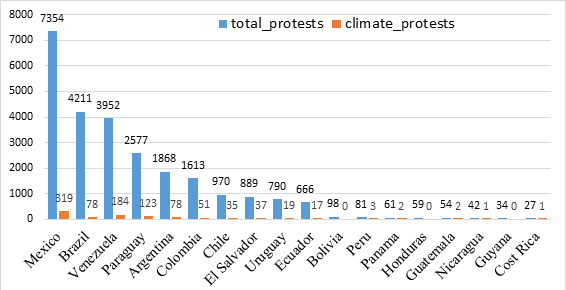
\includegraphics[width=3in,height=1.8in] {figures/climate/GSR_Climate_total.png}
		\label{fig:GSR_climate_number}
	}
	\subfigure[]{
		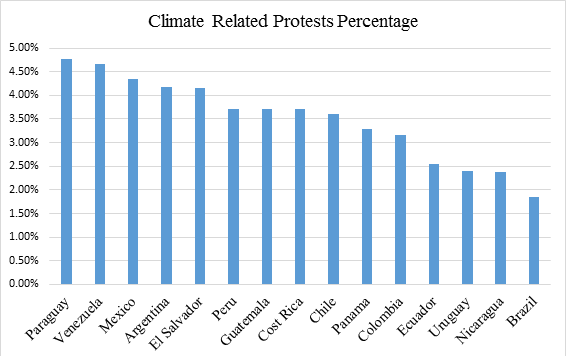
\includegraphics[width=3in,height=1.8in] {figures/climate/Climate_percentage.png}
		\label{fig:Climate_percentage}
	}	
	\caption{(a) GSR protest event distributions, (b) climate related protest percentage.}
\label{fig:total_climate}
\end{figure}

\begin{figure}[th]
	\centering
	\subfigure[]{
		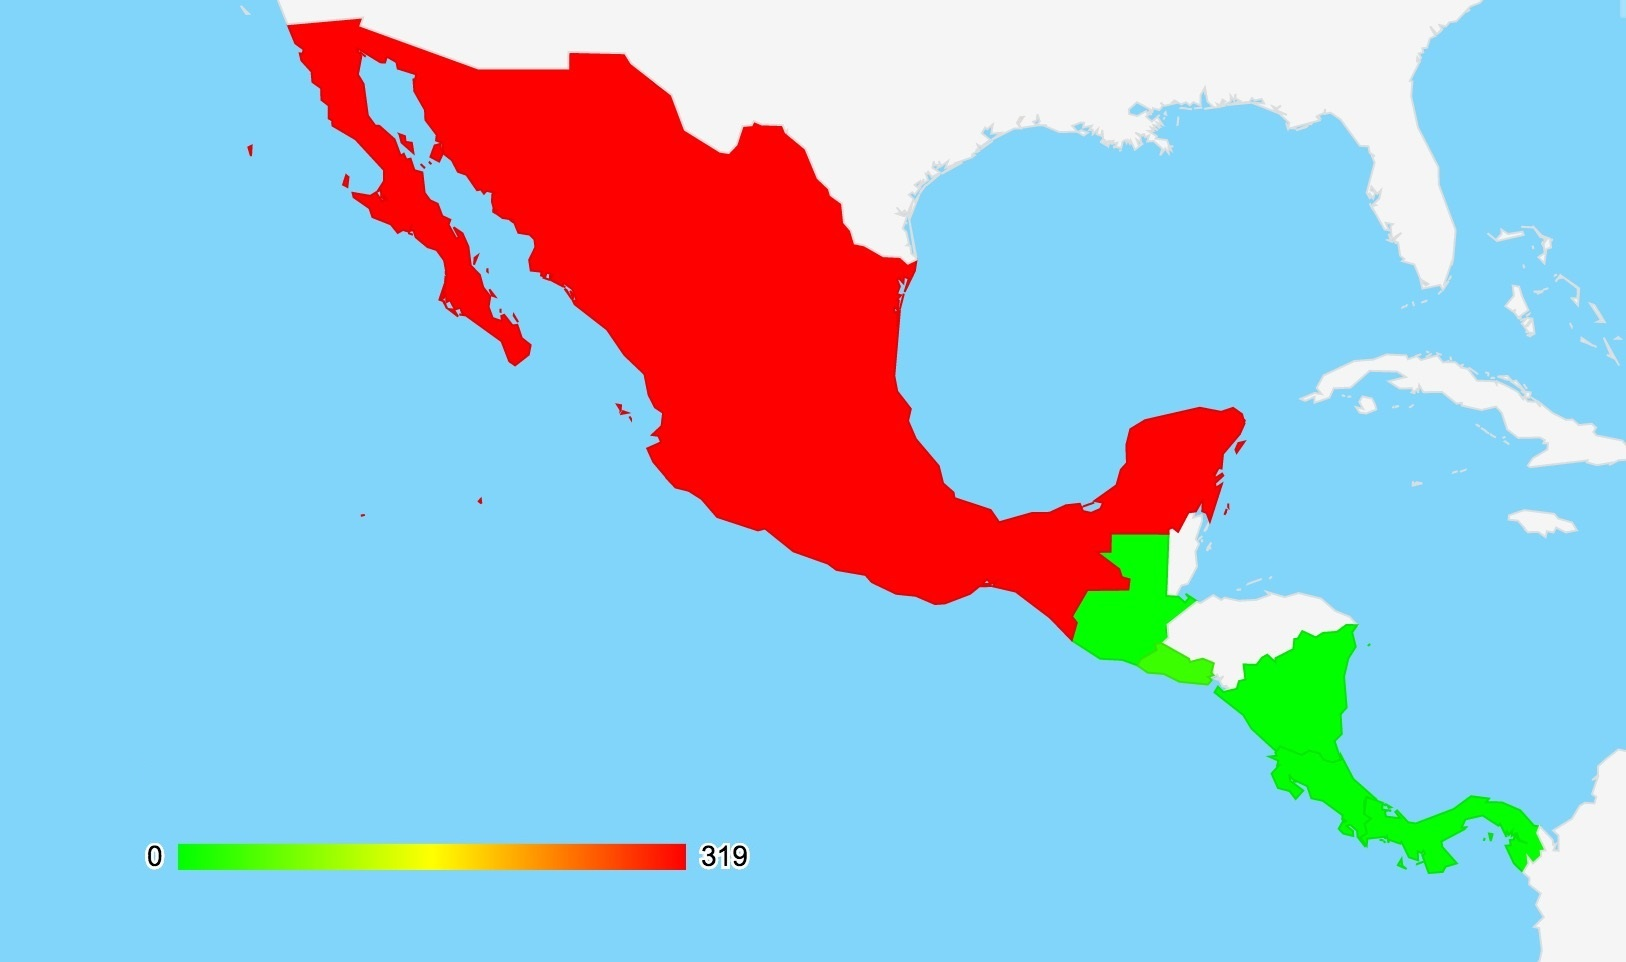
\includegraphics[width=2.8in] {figures/climate/WeatherProtest2.png}
		\label{fig:climate_weather_map2}
	}
	\subfigure[]{
		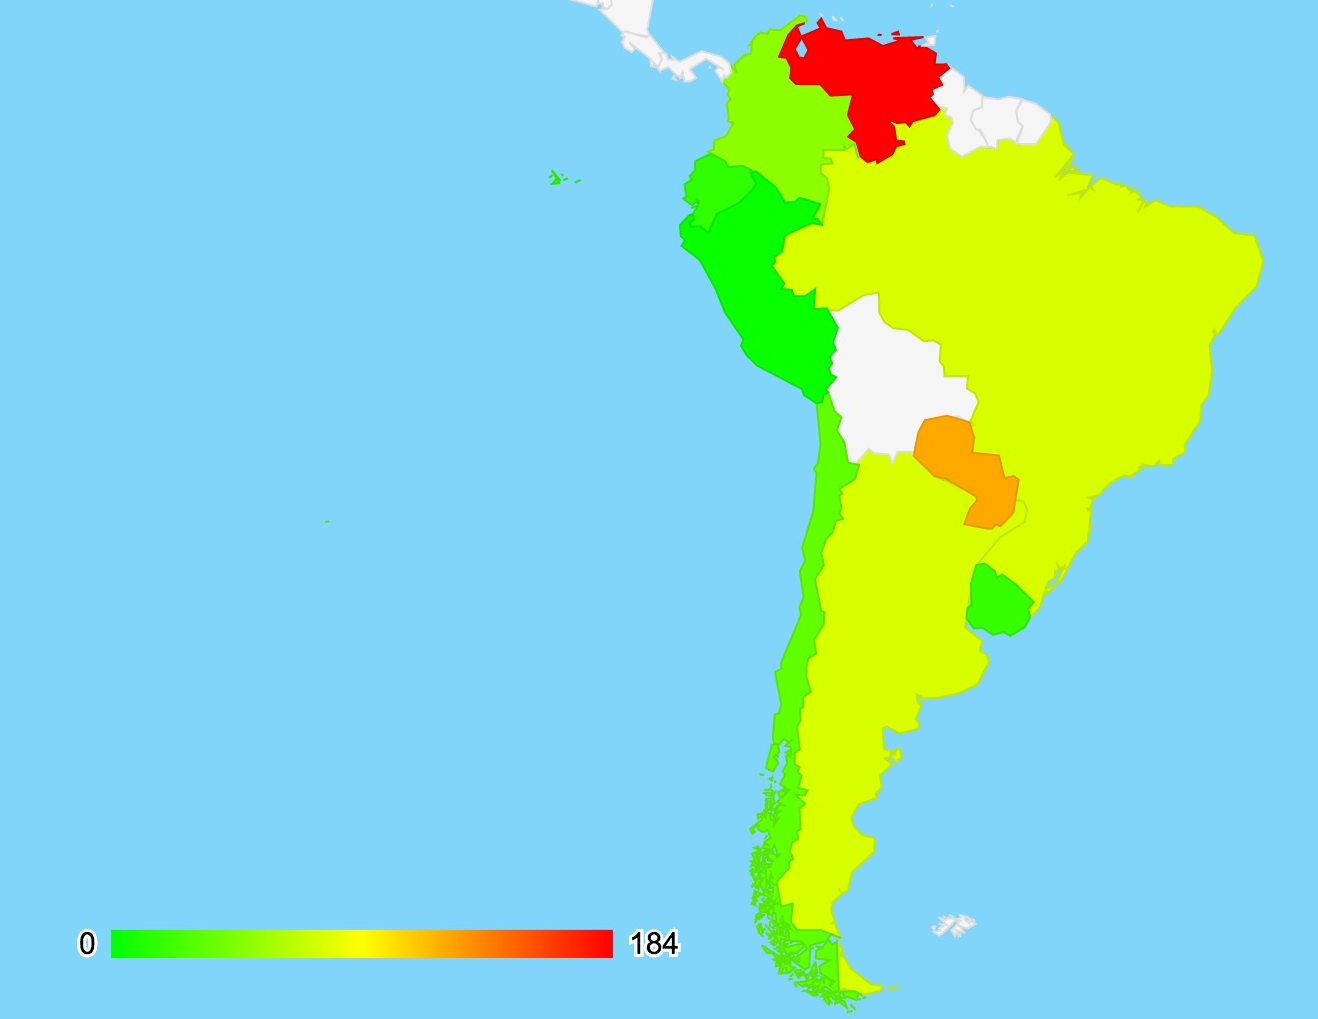
\includegraphics[width=2.8in] {figures/climate/WeatherProtest1.png}
		\label{fig:climate_weather_map1}
	}	
	\subfigure[]{
		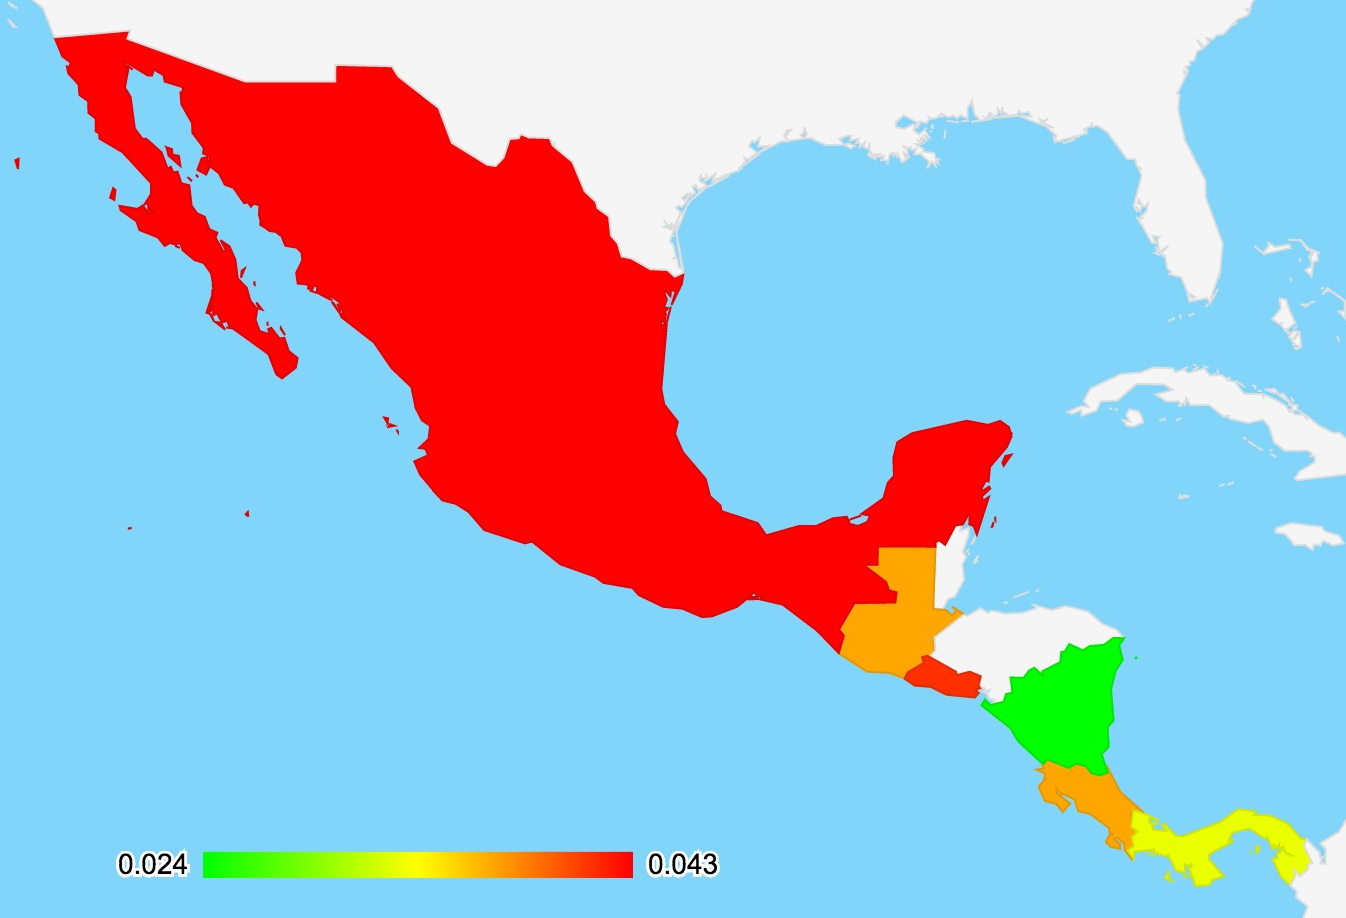
\includegraphics[width=2.8in] {figures/climate/Percentage2.png}
		\label{fig:GSR_Percentage2}
	}
	\subfigure[]{
		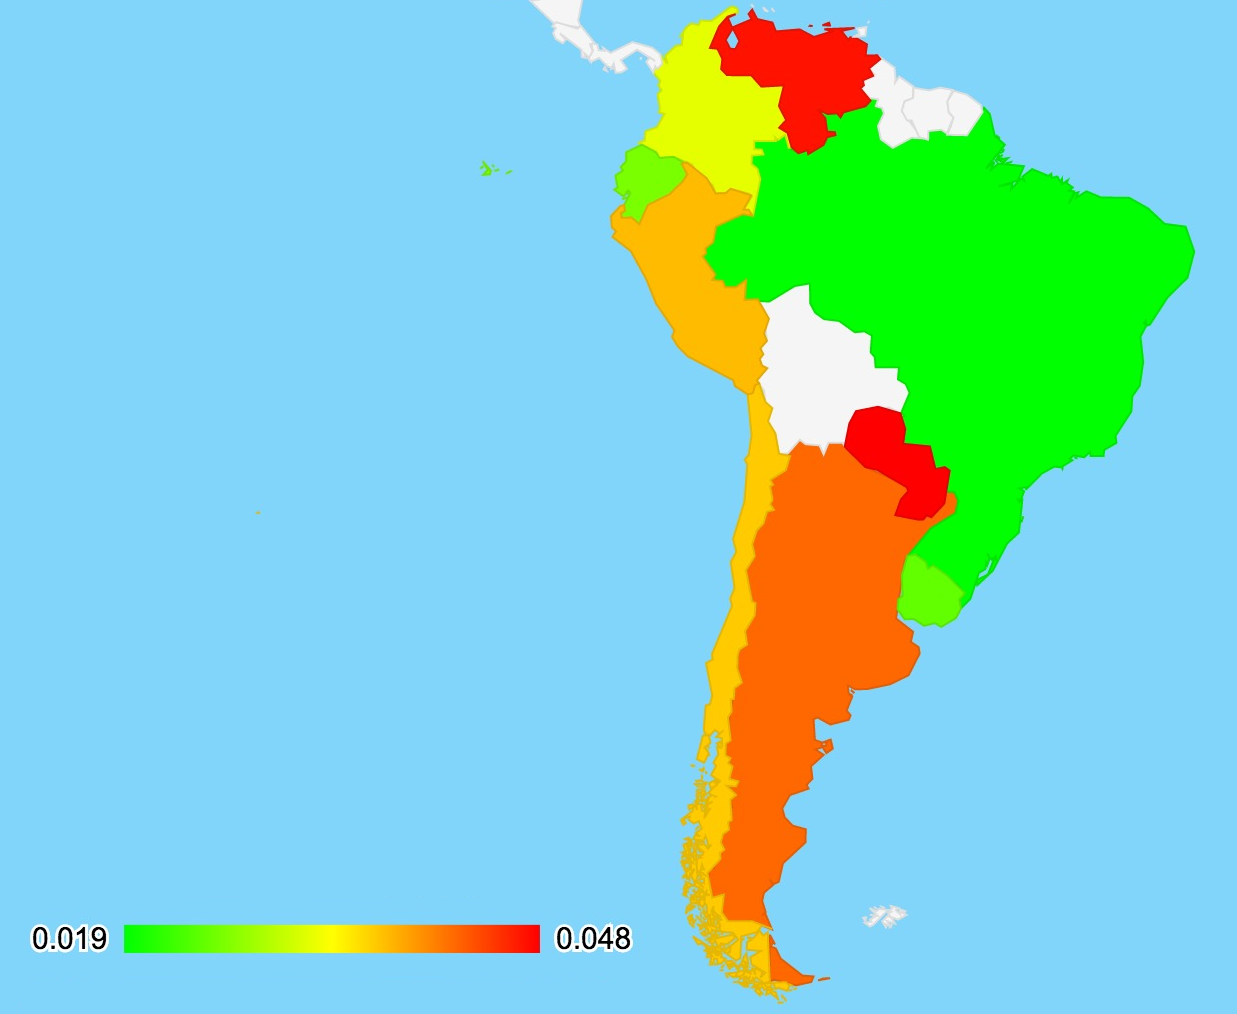
\includegraphics[width=2.8in] {figures/climate/Percentage1.png}
		\label{fig:Climate_Percentage1}
	}
	\caption{(a)(b) Climate protest events in South America. (c)(d) Climate protest percentage in South America.}
\label{fig:map_climate_no}
\end{figure}

%
%\begin{figure}[th]
%	\centering
%	\subfigure[]{
%		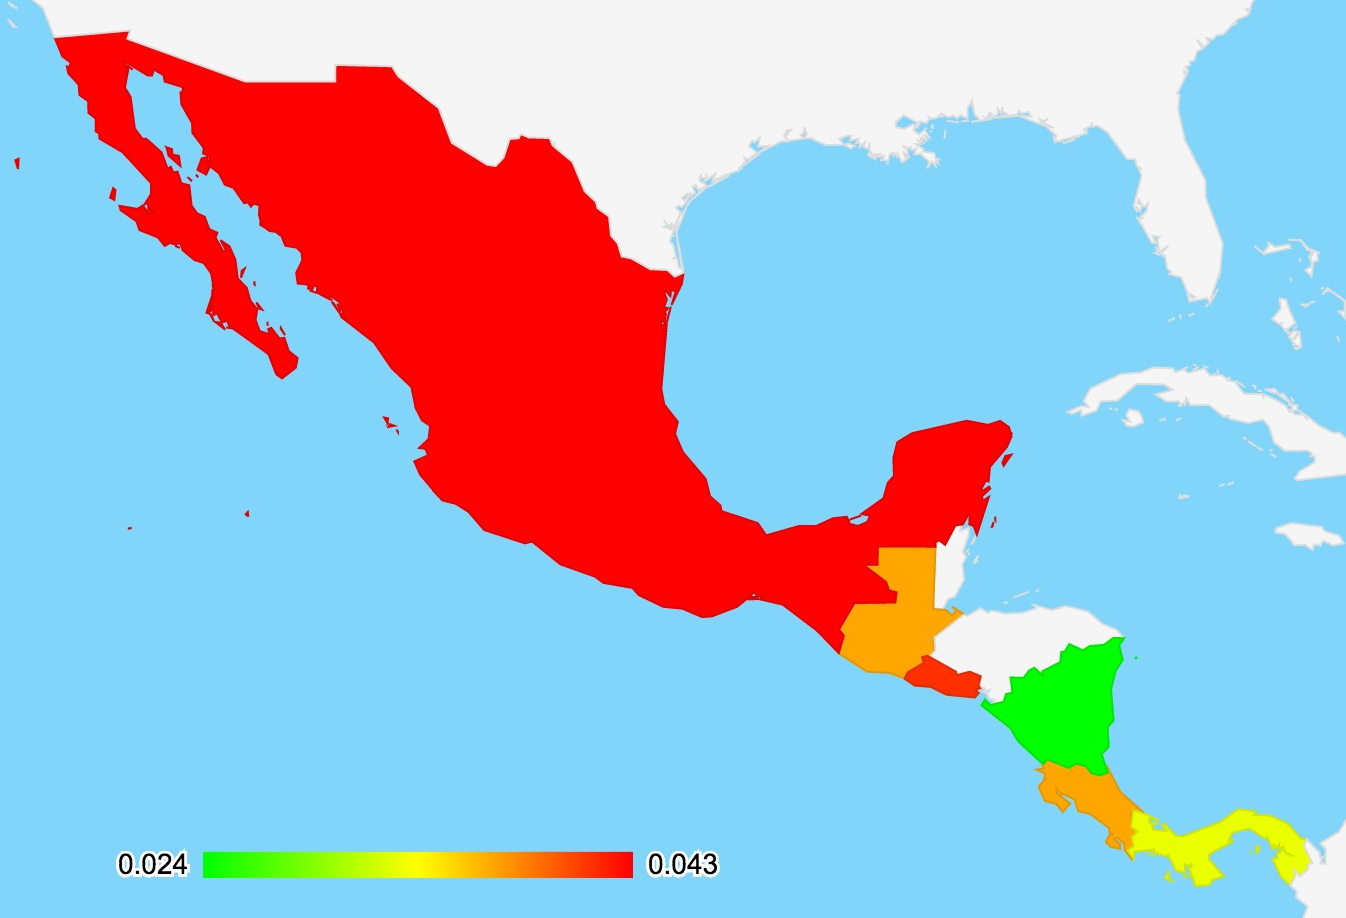
\includegraphics[width=2.8in] {figures/climate/Percentage2.png}
%		\label{fig:GSR_Percentage2}
%	}
%	\subfigure[]{
%		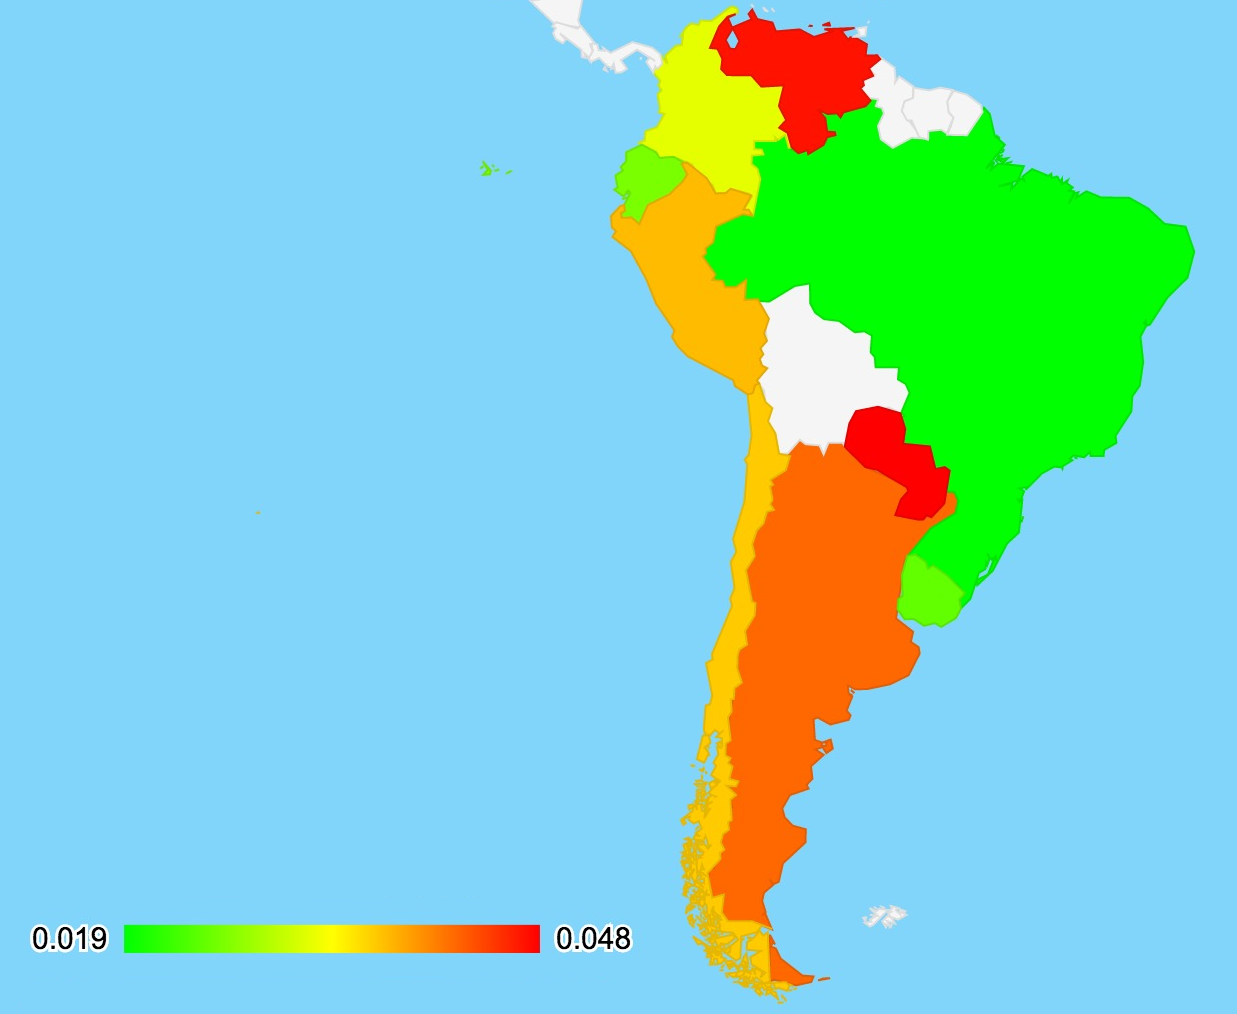
\includegraphics[width=2.8in] {figures/climate/Percentage1.png}
%		\label{fig:Climate_Percentage1}
%	}	
%	\caption{Climate protest percentage in South America.}
%\label{fig:map_percentage}
%\end{figure}

We study 25352 GSR events across South American counties from Jan, 2011 to March, 2015. Among all the 25352 GSR events, 974 events are classified into climate-related events, which is equal to 3.84\%. The GSR protest events and climate-related protests events for each country is plotted in Figure~\ref{fig:total_climate}. Mexico has both the largest GSR protest events and climate-related protest events. However, in terms of the percentages of the climate-related events, Paraguay is the highest (4.7\%) and Bolivia is the lowest (1\%). To have an overview of climate protests events distribution, we plot the climate protest events and its percentage over GSR in Figure~\ref{fig:map_climate_no}. It is important to evaluate how climate-related events has varied and changed in the past. We plot the monthly climate-related events and the percentages of climate-related protest events for each country in Figure~\ref{fig:climate_percentage}.




\begin{figure}[th]
	\centering
	\subfigure[]{
		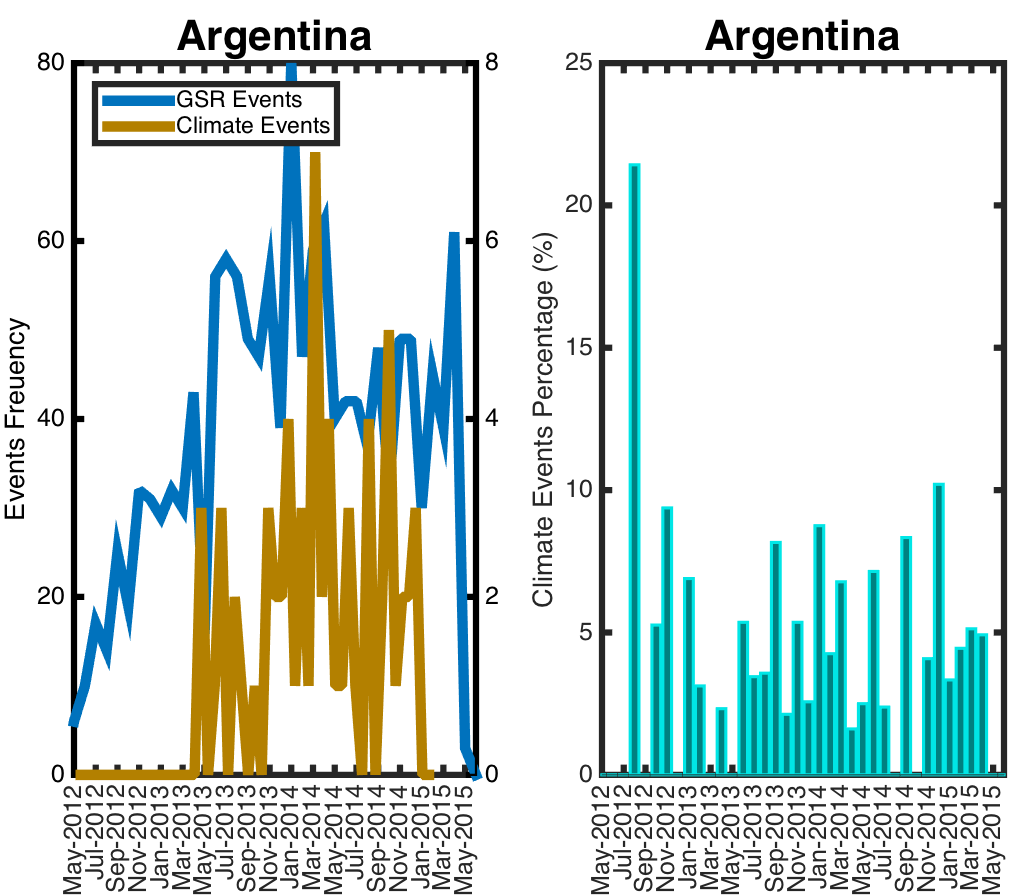
\includegraphics[width=3in,height=1.95in] {figures/climate/Argentina_percentage.png}
		\label{fig:percentage_Argentina}
	}
	\subfigure[]{
		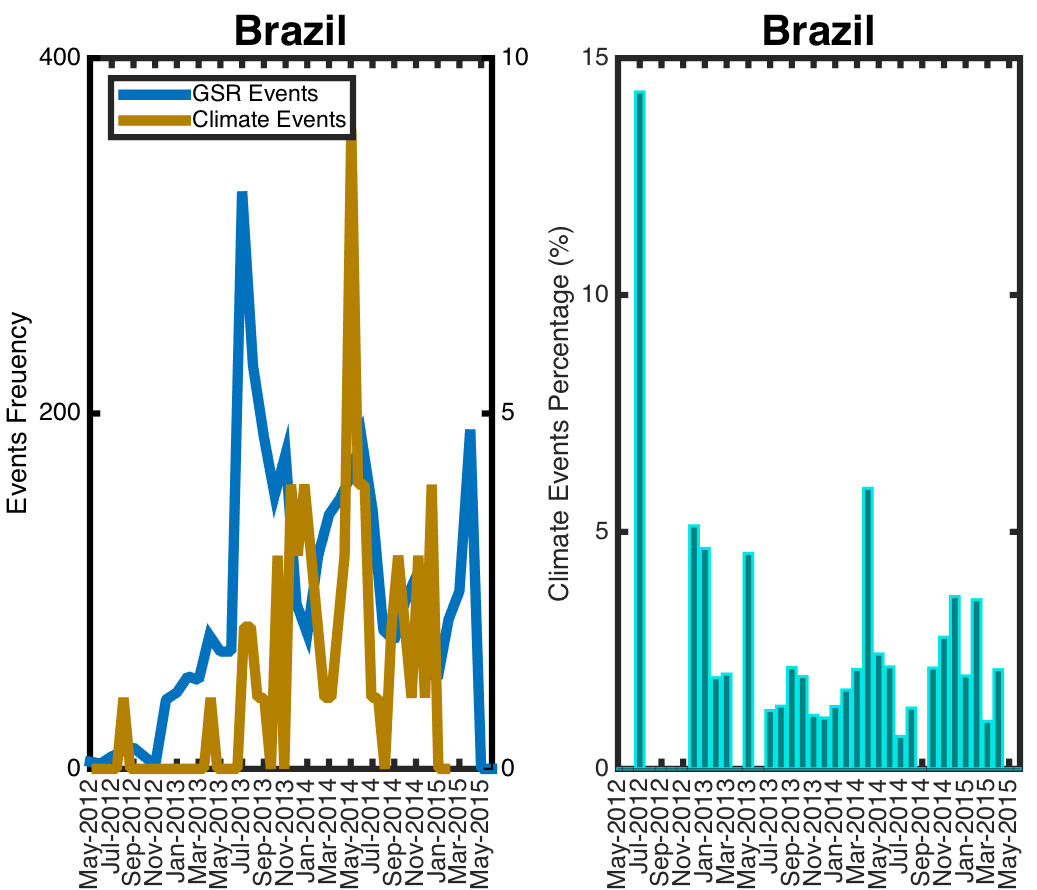
\includegraphics[width=3in,height=1.95in] {figures/climate/Brazil_percentage.png}
		\label{fig:percentage_Brazil}
	}	
	\subfigure[]{
		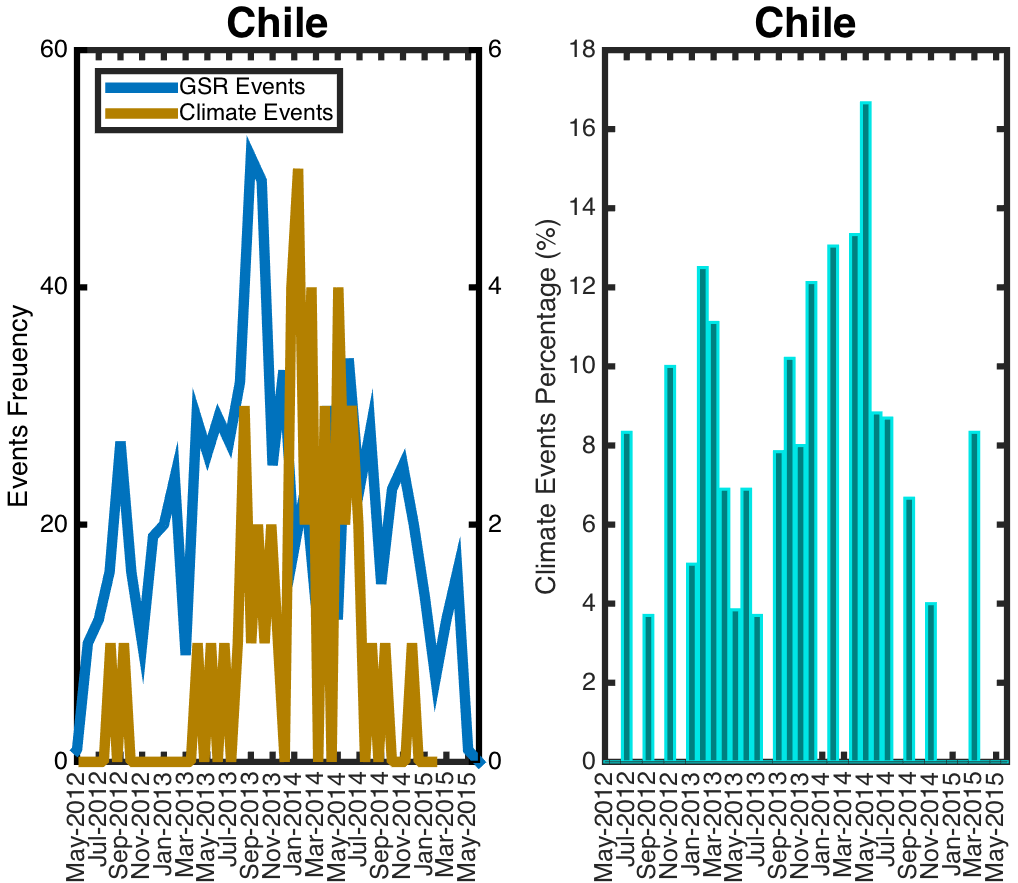
\includegraphics[width=3in,height=1.95in] {figures/climate/Chile_percentage.png}
		\label{fig:percentage_Chile}
	}
	\subfigure[]{
		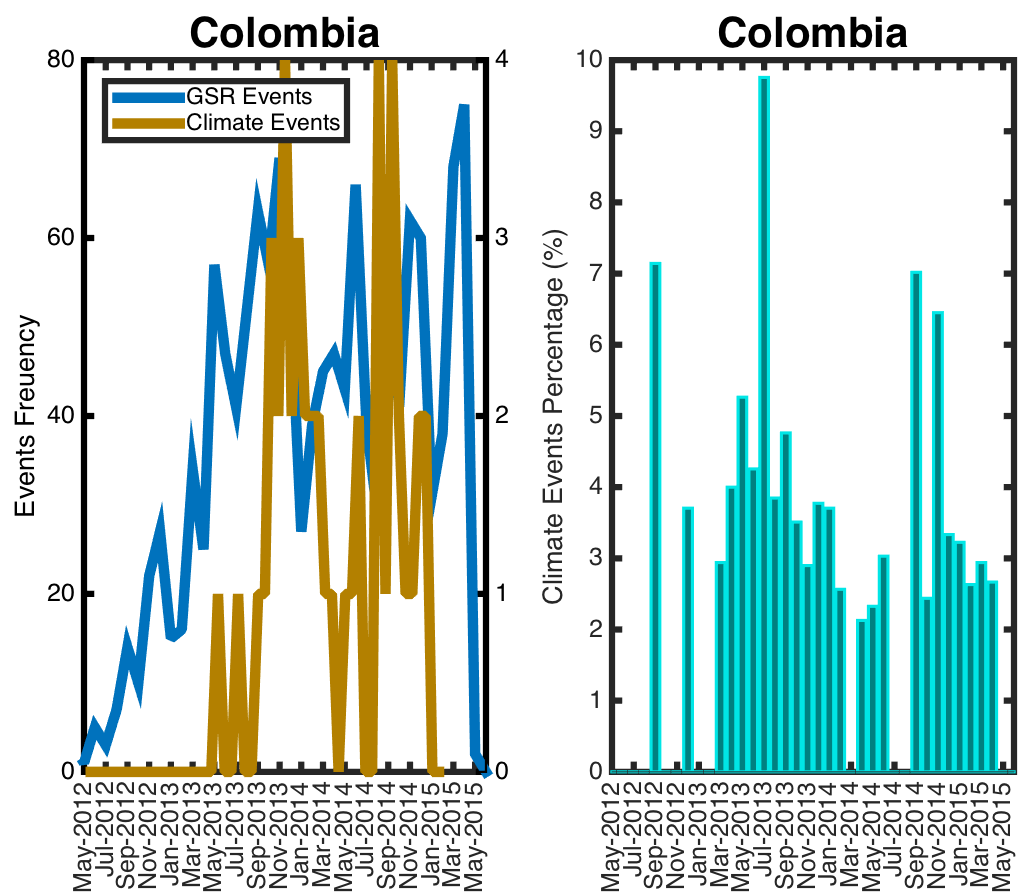
\includegraphics[width=3in,height=1.95in] {figures/climate/Colombia_percentage.png}
		\label{fig:percentage_Colombia}
	}
	\subfigure[]{
		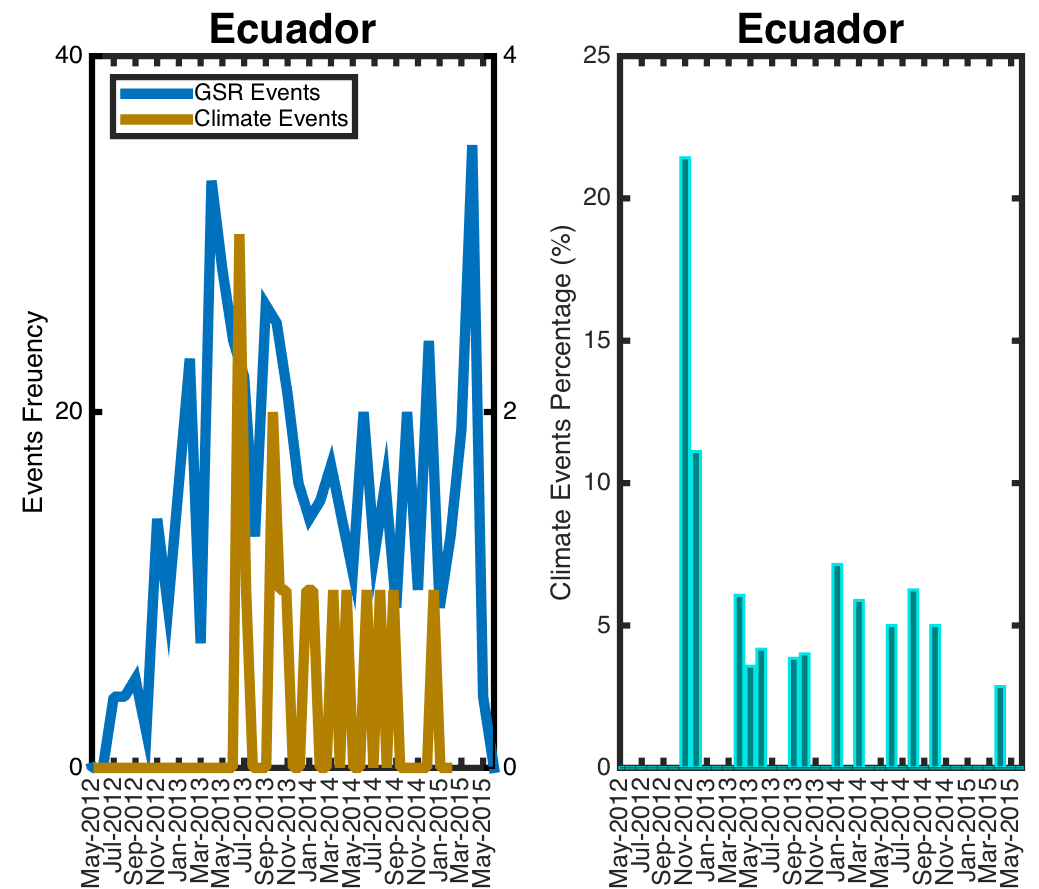
\includegraphics[width=3in,height=1.95in] {figures/climate/Ecuador_percentage.png}
		\label{fig:percentage_Ecuador}
	}
	\subfigure[]{
		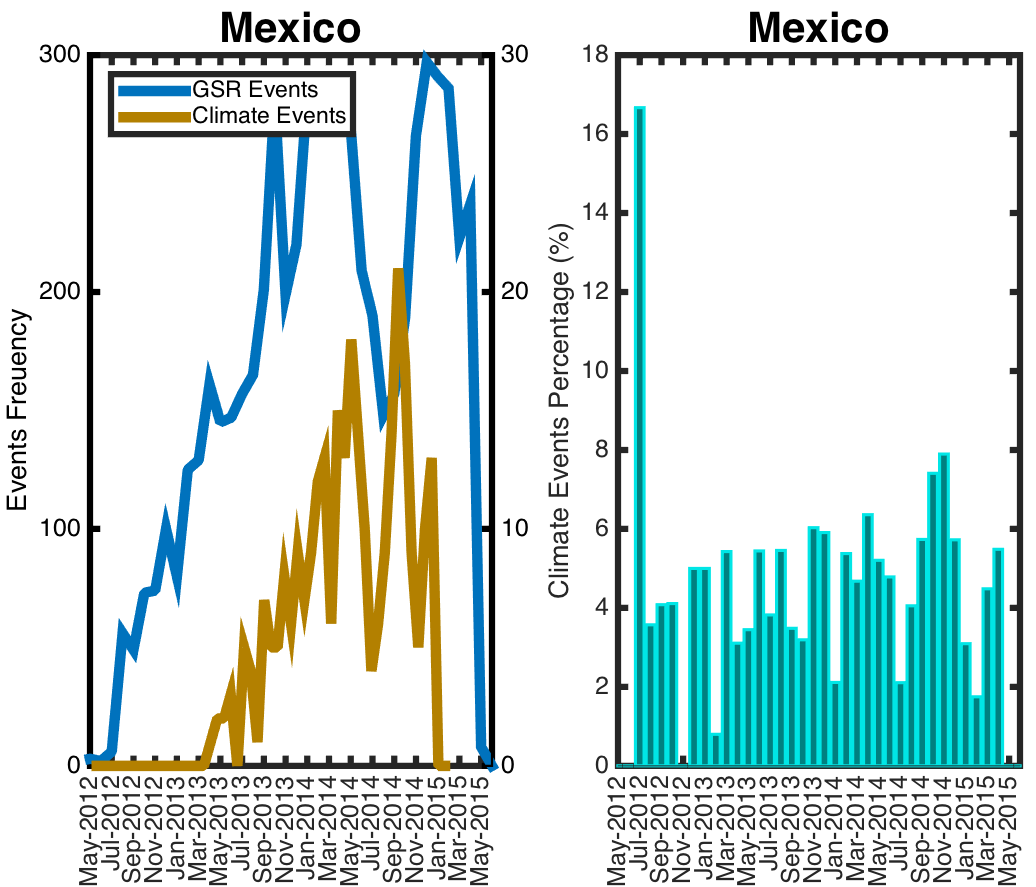
\includegraphics[width=3in,height=1.95in] {figures/climate/Mexico_percentage.png}
		\label{fig:percentage_Mexico}
	}
	\subfigure[]{
		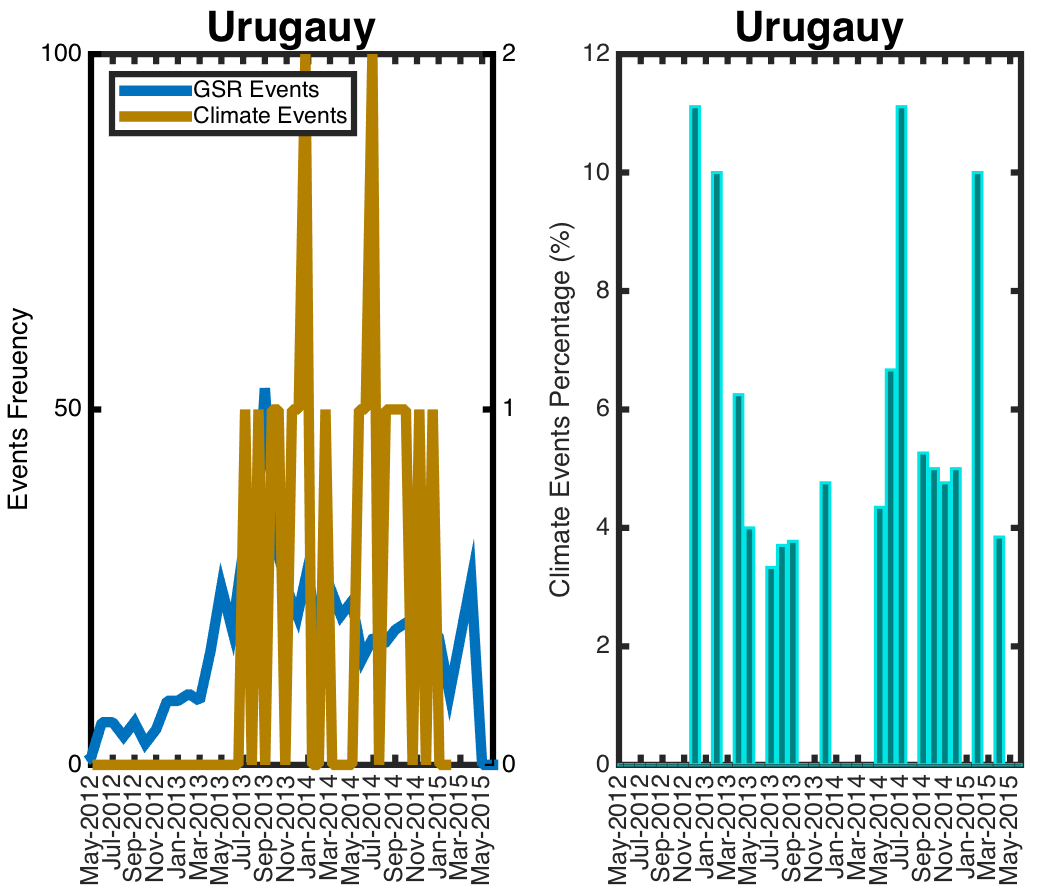
\includegraphics[width=3in,height=1.95in] {figures/climate/Urugauy_percentage.png}
		\label{fig:percentage_Urugauy}
	}
	\subfigure[]{
		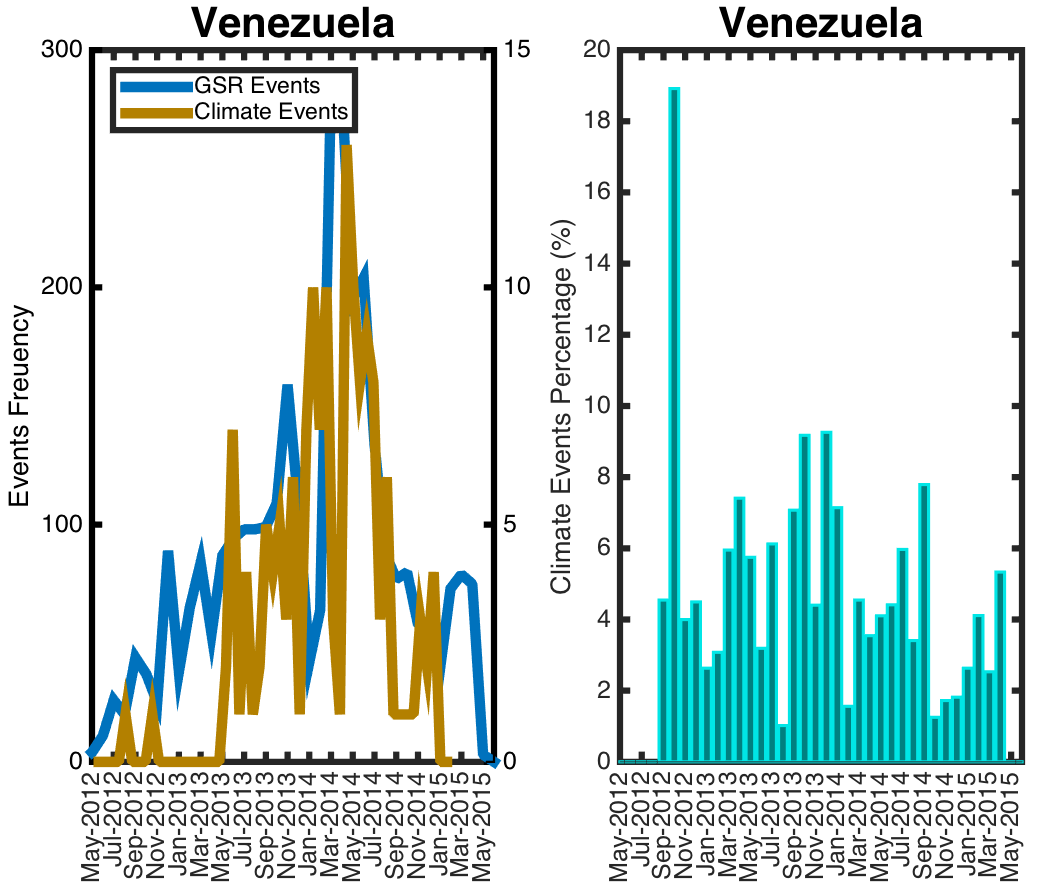
\includegraphics[width=3in,height=1.95in] {figures/climate/Venezuela_percentage.png}
		\label{fig:percentage_Venezuela}
	}
	\caption{Compare GSR events, climate events and climate events percentage of South American.}
\label{fig:climate_percentage}
\end{figure}



GSR event defines six different protest event types according to the concerns of people involved, they are employment, housing, energy \& resources, economic polices, other government policies, other. We are interested to see which event type is most dominant of all the climate related protest events. We plot the event type distributions for each country in Figure~\ref{fig:climate_eventType}.

%As we can see that even each county has different number of climate-related events, however, the distributions of event type are roughly the same, which means the type 011 has the highest percentages while type 016 the lowest.

\begin{figure}[t]
	\centering
	\subfigure[]{
		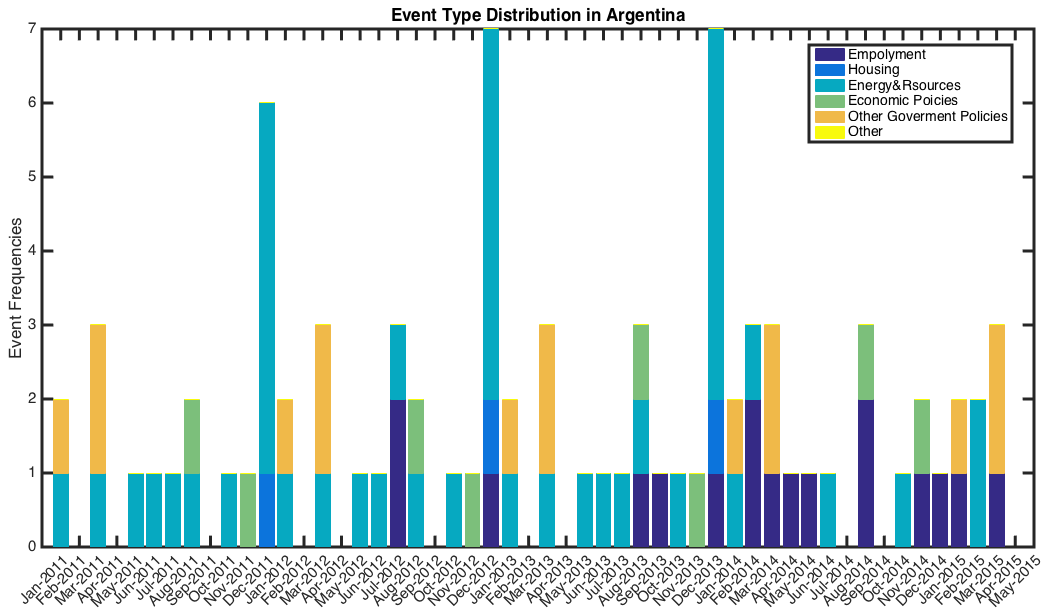
\includegraphics[width=3in,height=1.8in] {figures/climate/Argentina_type.png}
		\label{fig:type_Argentina}
	}
	\subfigure[]{
		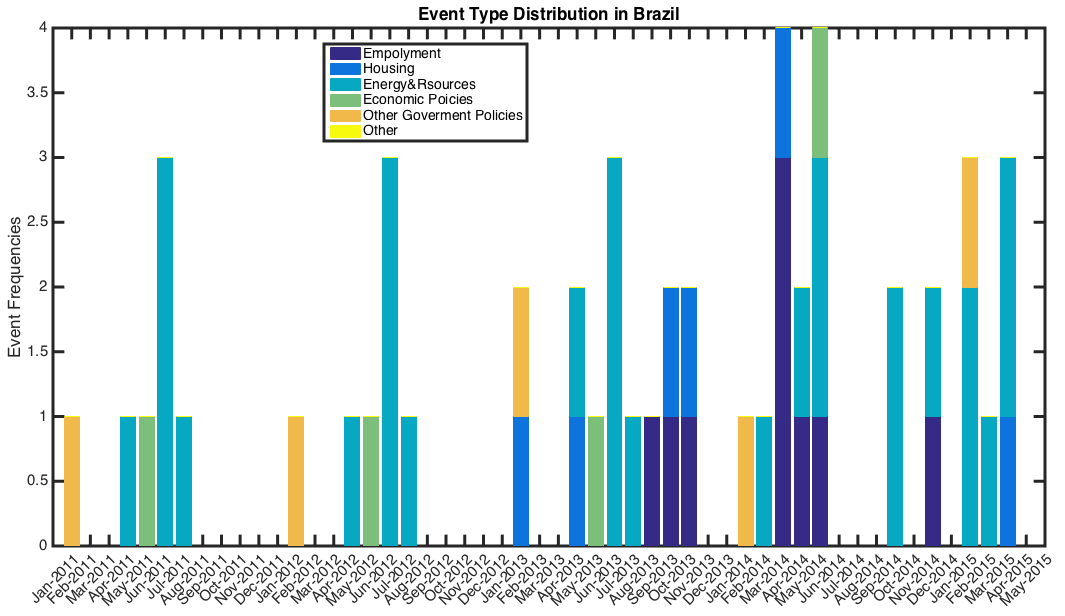
\includegraphics[width=3in,height=1.8in] {figures/climate/Brazil_type.png}
		\label{fig:type_Brazil}
	}	
	\subfigure[]{
		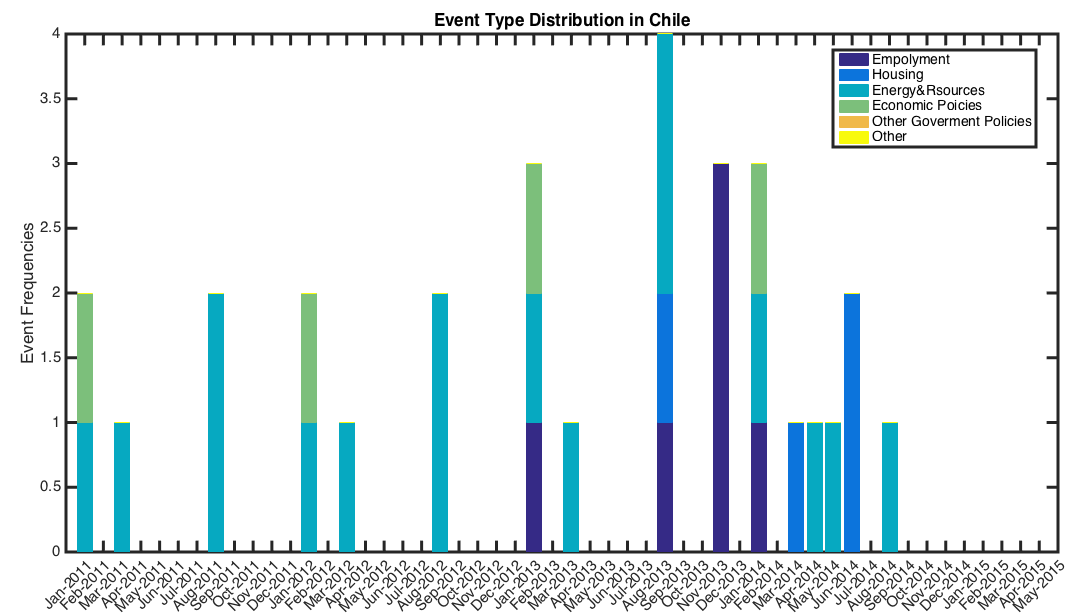
\includegraphics[width=3in,height=1.8in] {figures/climate/Chile_type.png}
		\label{fig:type_Chile}
	}
	\subfigure[]{
		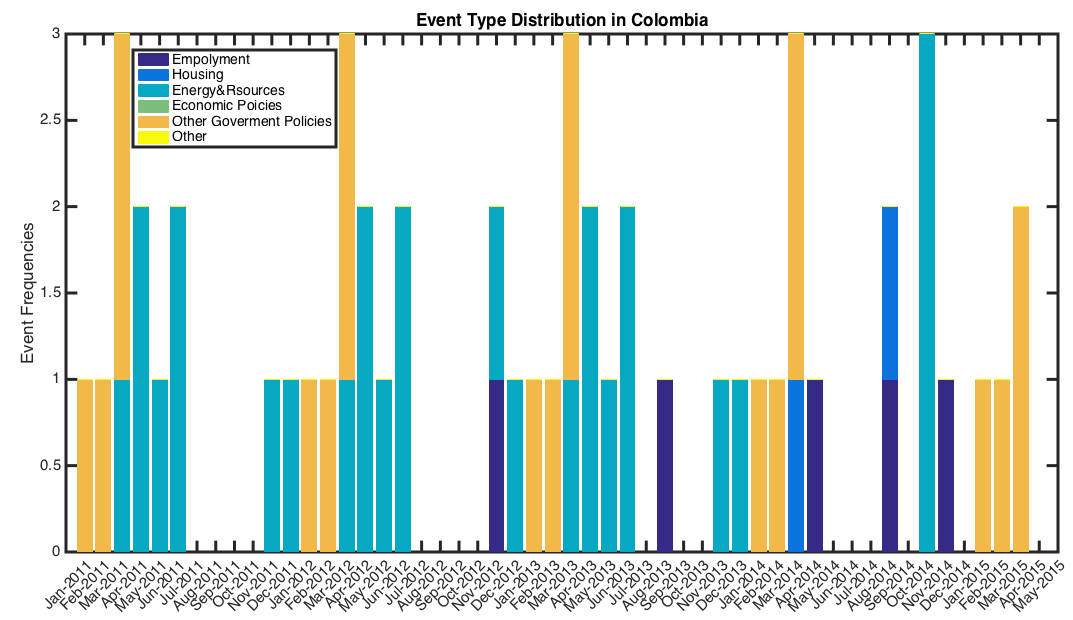
\includegraphics[width=3in,height=1.8in] {figures/climate/Colombia_type.png}
		\label{fig:type_Colombia}
	}
	\subfigure[]{
		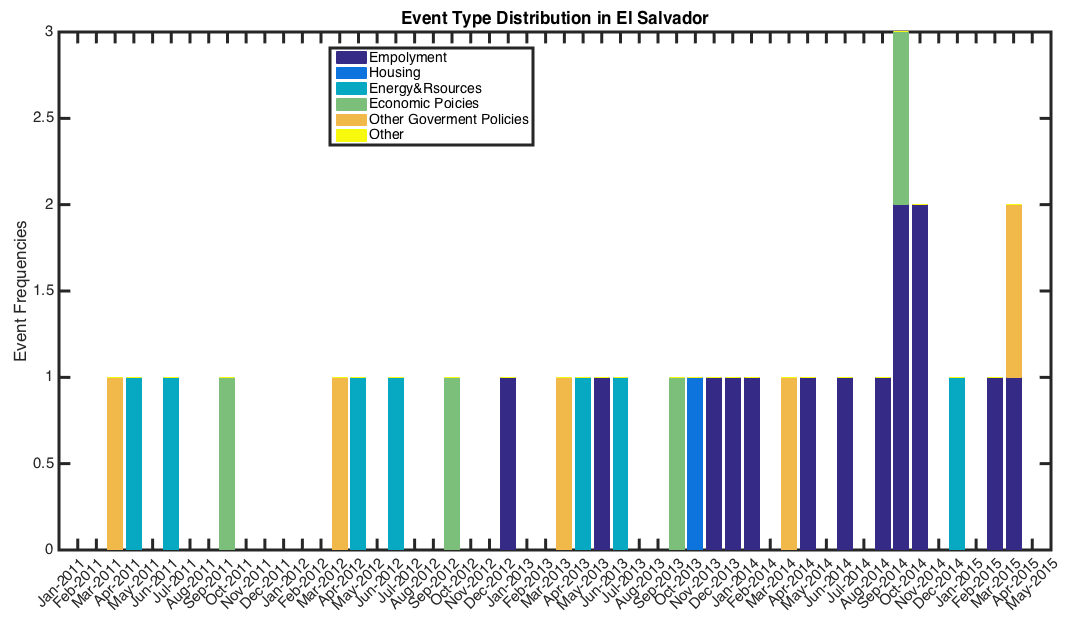
\includegraphics[width=3in,height=1.8in] {figures/climate/Elsd_type.png}
		\label{fig:type_Elsd}
	}
	\subfigure[]{
		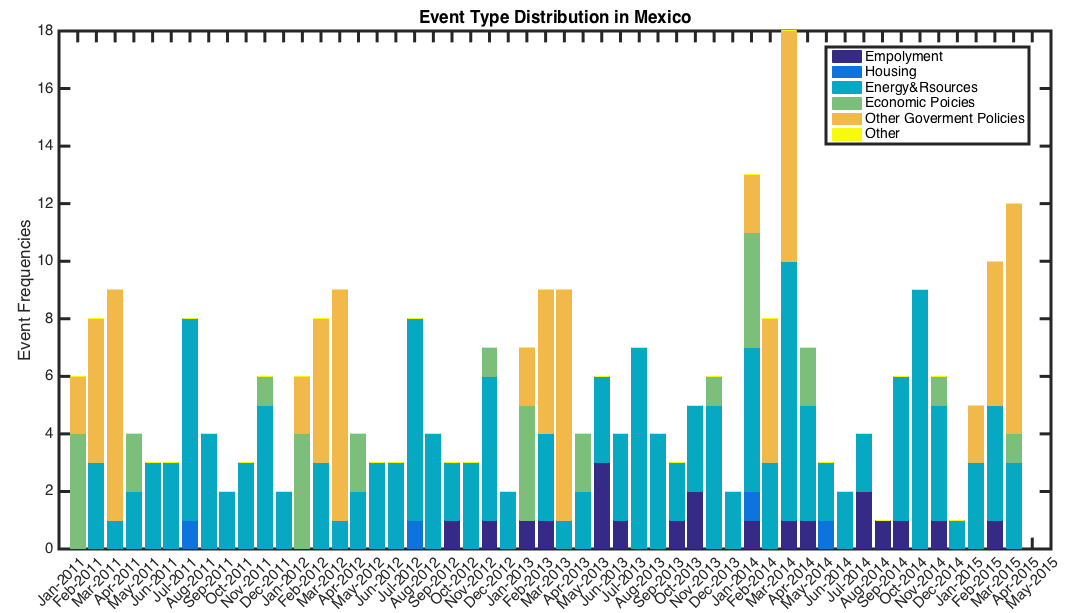
\includegraphics[width=3in,height=1.8in] {figures/climate/Mexico_type.png}
		\label{fig:type_Mexico}
	}
	\subfigure[]{
		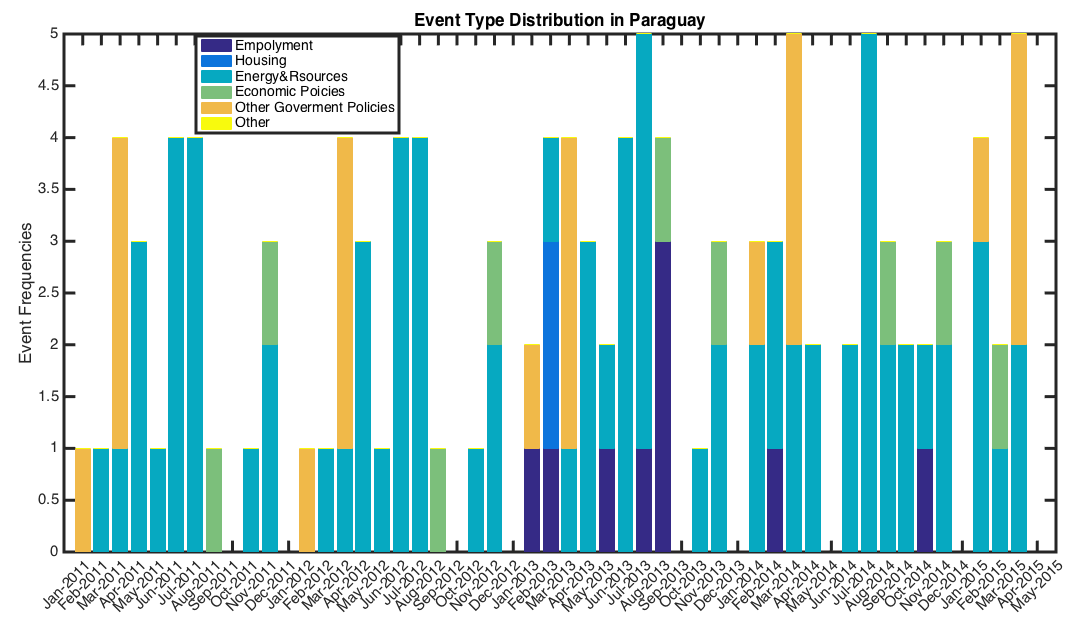
\includegraphics[width=3in,height=1.8in] {figures/climate/Paraguay_type.png}
		\label{fig:type_Paraguay}
	}
	\subfigure[]{
		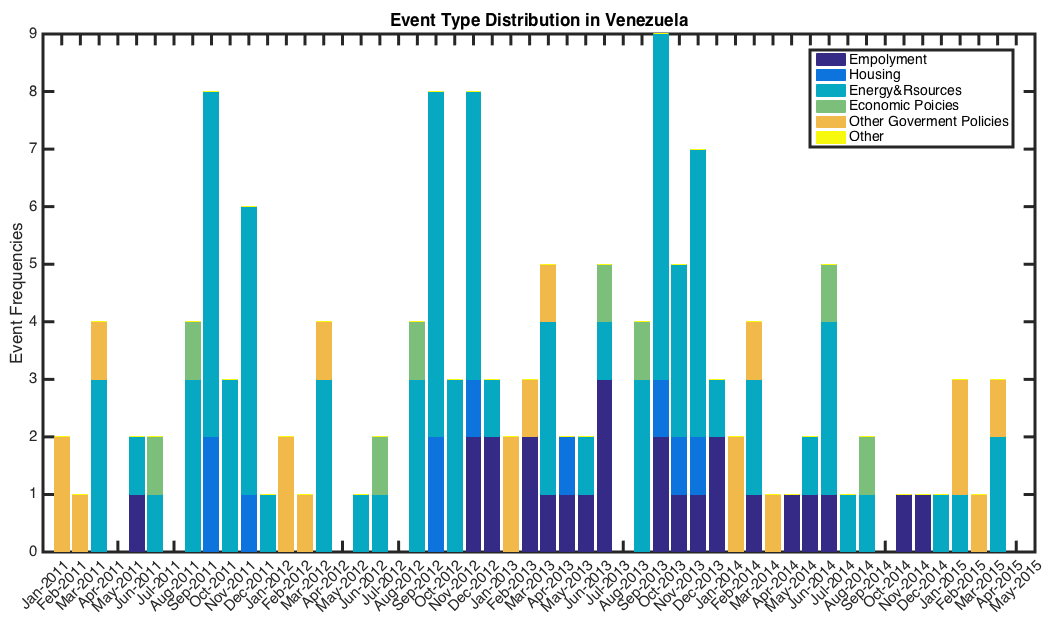
\includegraphics[width=3in,height=1.8in] {figures/climate/Venezuela_type.png}
		\label{fig:type_Venezuela}
	}
	\caption{Event type distribution of climate events for South American.}
\label{fig:climate_eventType}
\end{figure}

\subsection{Information Chain}
The story telling algorithm we employed is based on weighted scores of similarities across news articles for three sets of features: textual features (related to keywords), spatial features (such as locations and geographical coordinates), and actors (such as person(s), and organizations mentioned in the articles)~\cite{ninguncovering}. The chaining methodology is developed with the goal of identifying all documents related to a climate change story and to keep track of the news story as new documents arrive. Documents belonging to such a chain cover the same event and are ordered by time. The algorithm operates in an incremental fashion wherein every new input article is analyzed as it arrives and is appended to already existing chain(s). This analysis involves a two-step process. In the first step, we compare an incoming article Di to articles from the last n1 days to identify the most similar articles and then designate candidate chains to which the current article can be attached to. If no similar articles are found, then a new chain is created with this article as a seed.
Further, to assess if two documents are referring to the same underlying context, we calculate their similarity scores with respect to three features:
- textual features,
- spatial features, and
- actors.

The storytelling algorithm is employed to track the evolvement process of a climate event, from its beginning to its ending, and finally develop into a civil unrest event. To avoid confusion, we build story chains country by country. We collect each country�s RSS news from its top leading news agencies, for instance, Brazil news comes from Brazil� O Globo, Estadao, and Jornal do Brasil. In addition to this data, we also have access to a human curated list of civil unrest events that happened during this period. This list, called the Gold Standard Report (GSR) described in~\cite{ramakrishnan2014beating}, contains news reports for each event from the three major news sources. For each country�s document stream, we employ storytelling algorithm. The following shows some story chains for climate related protest events.

\begin{figure}[th]
	\centering
	\subfigure[]{
		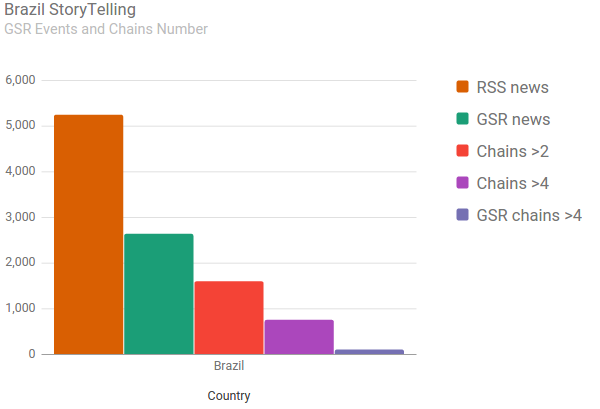
\includegraphics[width=3in,height=2.1in] {figures/climate/Brazil_story_bar.png}
		\label{fig:Brazil_story1}
	}
	\subfigure[]{
		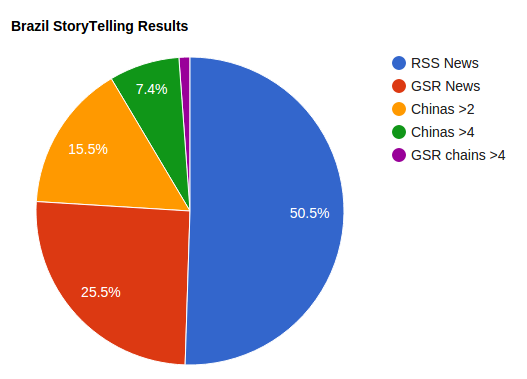
\includegraphics[width=3in,height=2.1in] {figures/climate/Brazil_story_pie.png}
		\label{fig:Brazil_story2}
	}	
	\caption{Story chain overview of Brazil protests events.}
\label{fig:Brazil_storytelling}
\end{figure}



\begin{figure}[th]
	\centering
	\subfigure[]{
		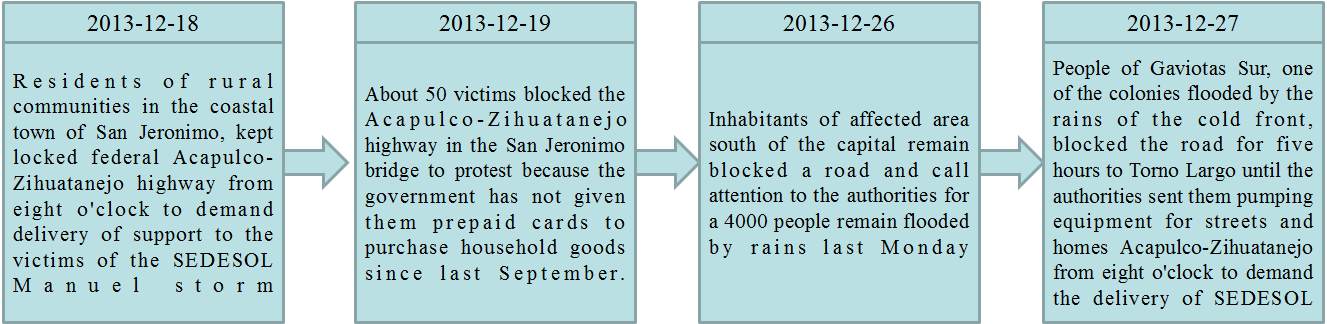
\includegraphics[width=5in,height=1.5in] {figures/climate/Mexico_hurricane.png}
		\label{fig:Mexico_story}
	}
	\subfigure[]{
		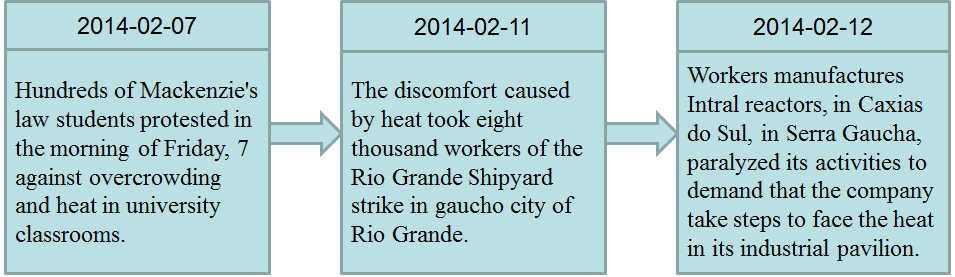
\includegraphics[width=5in,height=1.3in] {figures/climate/Brazil_heat.png}
		\label{fig:Brazil_story}
	}	
	\subfigure[]{
		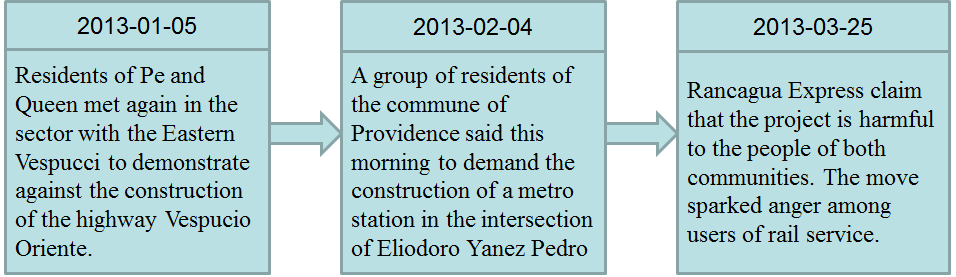
\includegraphics[width=5in,height=1.3in] {figures/climate/Chile-construction.png}
		\label{fig:Chile_story}
	}	
	\caption{Story chain for (a) Mexico hurricane climate events. (b) Brazil heat wave events. (c) Chile anti-construction events.}
\label{fig:storytelling}
\end{figure}



%\subsection{Dynamic Flow in Twitter}



%We know climate changes can cause health, economic problems, but will that effect the society stabilization, if so, how large extent?
%
%Create a database of climate change extreme weather keywords. We can also use DQE to generate more keywords, in Spanish and Portuguese.
%Filter the GSR descriptions, see how many GSR events talking about climate related words, what are their categories.
%
%Different countries civil unrest may be influenced under different climate change scenarios.
%
%Find the evidence for climate influence civil unrest
%Run storytelling
%
%
%There is a problem, given initial keywords, the DQE will capture protests which are non-climate related protests. Shall we filter those non-climate protests or keep it? Thanks!
%
%1. improve storytelling procedure, get more interesting results
%2. cluster DQE based on spatial information, to show DQE word cloud results (drought, storm) at different locations.
%3. build filter / classifier, to get the precise climate protests events in each country
%4. start to write the climate chapter, because visualization like map plotting also takes a lot of time.
